

\section{Generative Model}

    \textbf{Discriminative:} $p(y|x)$ 
    \textbf{Generative:} $p(x, y)$ \\
    Can derive condi. from joint distr., but not vice versa!

    \textbf{Generative models for classification:}\\
    1. $P(X,Y) = P(X)P(Y|X)$ \\ density over inputs, probabilistic classifier\\
    2. $P(X,Y) = P(Y)P(X|Y)$ \\ prior over classes, appearence for each class\\

\subsection{Bayes Classifier (supervised)}\

    % 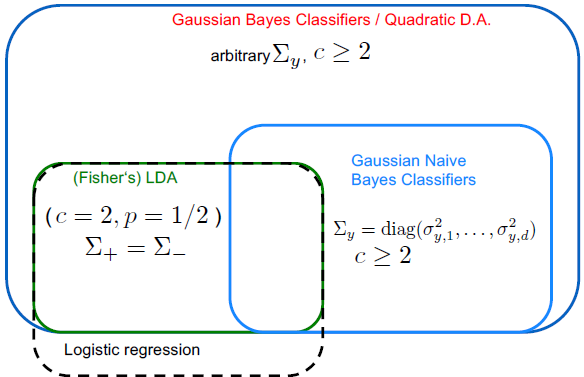
\includegraphics[width=0.5\linewidth]{pics/1.png}\\ % !改!!!!!!!!!!!!!!!!!!!!!!!

    \textbf{Naive Bayes Model:} 
    class prior: $P(Y=y) = p_y \, y \in \mathcal{Y} = \{1, \cdots , c \}$ \\
    features as conditionally independent given $Y$: $P(X_1, \cdots , X_d|Y) = \prod_{i=1}^d P(X_i|Y)$
    
    \textbf{Gaussian NBC:} \textbf{continuous} RV \\
    \textit{Learning:} 1. MLE: $P(Y=y) = \frac{Count(Y=y)}{n}$ \\ 
    2. MLE: $P(x_i|y) = \mathcal{N}(x_i|\mu_{y,i}, \sigma_{y,i}^2)$\\
    $\hat{\mu}_{y,i} = \frac{1}{Count(Y=y)} \sum_{j: y_j=y} x_{j,i}$
    $\sigma_{y,i}^2 = \frac{1}{Count(Y=y)} \sum_{j: y_j=y} (x_{j,i} - \hat{\mu}_{y,i})^2$\\
    \textit{Prediction:} $y = \mathrm{argmax}_{y'}\, P(y'|x) = \mathrm{argmax}_{y'}\, P(y')\prod_{i=1}^d P(X_i|Y)$

    \textbf{Categorical NBC:} \textbf{discrete} RV \\
    \textit{Learning:} 1. MLE: $P(Y=y) = \frac{Count(Y=y)}{n}$ \\ 
    2. MLE: $P(X_i = x|Y = y) = \theta_{x|y}^{(i)} = \frac{Count(X_i = x, Y = y)}{Count(Y = y)}$\\
    \textit{Prediction:} $y = \mathrm{argmax}_{y'}\, P(y'|x) = \mathrm{argmax}_{y'}\, P(y')\prod_{i=1}^d P(X_i|Y)$

    \textbf{Decision rules for binary classification:} Goal: $y = \mathrm{argmax}_{y'} P(y'|x) \Rightarrow y = sign(\mathrm{log} \frac{P(Y=1|x)}{P(Y=-1|x)})$

    \textbf{GNB, c=2, shared variance (= logistic regression = linear classifier):} \textit{discriminant function:} $f(x)=\mathrm{log} \frac{P(Y=1|x)}{P(Y=-1|x)} = w^Tx + w_0$,
    $w_i = \frac{\mu_{+, i} - \mu_{-, i}}{\sigma_{i}^2}$
    $w_0 = \mathrm{log} \frac{\hat{p}_+}{1-\hat{p}_+} + \sum_{i=1}^d \frac{\hat{\mu}_{-, i}^2 - \hat{\mu}_{+, i}^2}{2\hat{\sigma}_i^2}$

    Class distri.: $P(Y=1|x) = \frac{1}{exp(-f(x))} = \sigma (w^Tx+w_0)$

    \textbf{GBC:}
    class prior: $y \in \mathcal{Y} = \{1, \cdots , c \}$, $P(Y=y) = p_y = \frac{Count(Y=y)}{n}$ \\
    features as generated by multivariate Gaussian: $P(x|y) = \mathcal{N}(x;\mu_{y}, \Sigma_{y})$, 
    $\hat{\mu}_{y} = \frac{1}{Count(Y=y)} \sum_{i: y_i=y} x_{i}$
    $\Sigma_{y} = \frac{1}{Count(Y=y)} \sum_{i: y_i=y} (x_{i} - \hat{\mu}_{y})(x_{i} - \hat{\mu}_{y})^T$\\

    \textbf{Fisher's LDA:} $y = sign(f(x)) = sign(\boldsymbol{w}^T\boldsymbol{x} + w_0)$, $\boldsymbol{w} = \hat{\Sigma}^{-1} (\hat{\mu}_+ - \hat{\mu}_-)$, $w_0 = \frac{1}{2} (\hat{\mu}_-^T \Sigma^{-1} \hat{\mu}_- - \hat{\mu}_+^T \Sigma^{-1} \hat{\mu}_+)$

    \textbf{Conjugate priors:} \\
    Prior / Posterior \qquad Likelihood function\\
    Beta \qquad \qquad \qquad Bernoulli/Binomial\\
    Dirichlet \qquad \qquad Categorical/Multinomial\\
    Gaussian (fixed covariance) \qquad  Gaussian\\
    Gaussian-inverse Wishart \qquad  Gaussian\\
    Gaussian process \qquad  \qquad Gaussian\\


 \subsection{Gaussian Mixture Model (unsup.)}
    \textbf{Gaussian Mixture:} $P(x|\theta) = \sum_{y \in \{1, \cdots, i\ \cdots \}} \underbrace{w_i}_{p(y=i|\theta)}\cdot\underbrace{\mathcal{N}(x;\mu_i,\Sigma_i)}_{p(x|y=i,\theta)}$
    \vspace{-0.3cm}
    
    \textbf{Hard-EM Algorithm:}
    
    E-Step: Predict most likely class for each data point:\\
    $y_i^{(t)}=\mathrm{argmax}_yP(y|x_i,\theta^{(t-1)})=\mathrm{argmax}_y P(y|\theta^{(t-1)}) P(x_i|y,\theta^{(t-1)})$\\
    M-step: Compute MLE for GBC (closed form):\\
    \centerline{$\theta^{(t)}= \mathrm{argmax}_\theta P(D^{(t)}|\theta)$}
    Problem: Hard EM assigns a fixed label for uncertain x, even though the model is uncertain.\\
    Work poorly if clusters are \textbf{overlapping}
    
    \textbf{Soft EM:} \textit{\small(or just EM)}\\
    E-Step: Get cluster Membership with $\scriptstyle\mu^{(t-1)},\Sigma^{(t-1)},w^{(t-1)}$.\\
    \centerline{$\gamma_j(x) = P(y = j| x,\Sigma,\mu,w)= \frac{w_jP(x|\Sigma_j,\mu_j)}{\sum_l w_l P(x|\Sigma_l,\mu_l)}$}
    M-Step: Fit Clusters to weighted data points.\\
    \centerline{$w_j^{(t)}= \frac{1}{n}\sum_i\gamma_j^{(t)}(x_i);\;\mu_j^{(t)} = \frac{\sum_i\gamma_j^{(t)}(x_i)x_i}{\sum_i\gamma_j^{(t)}(x_i)}$}
    \centerline{$\Sigma_j^{(t)}= \frac{\sum_i\gamma_j^{(t)}(x_i)(x_i-\mu_j^{(t)})(x_i-\mu_j^{(t)})^T}{\sum_i \gamma_j^{(t)}(x_i)}$}

    \textbf{Initialization:} \textit{Weights:} typically uniform distr.; \textit{Means:} randomly initi./k-means++; \textit{Variances:} Spherical: $\Sigma_i = \sigma_i^2 I_d$, Diagonal: $\Sigma_i = diag(\sigma_1 = \cdots = \sigma_d)$, Tied: $\Sigma_1 = \cdots = \Sigma_k$
    
    \textbf{Degeneracy of GMM}: For \#Clusters = \#points the GMM overfits to $\mu=x$, $\sigma=0$. $\Rightarrow \text{ add } +\nu^2\mathbb{I}$ to the $\Sigma_j^{(t)}$ update.\\
    For semi-supervised GMM: Set $\gamma_j^{(t)}(x_i)= \mathbb m{1}_{\{j=y_i\}}$ for labeled data\\
    To select k=\#gaussians we can use cross-validation

    \textbf{Reasons mixture model useful:} 
    1. Can encode assumptions about “shape” of clusters 
    2. Can be part of more complex statistical models E.g., classifiers
    3. Probabilistic models can output likelihood $P(x)$ of a point $x$. (Useful for \textit{anomaly/outlier detection})
    4. Can be naturally used for semi-supervised learning
    
    \textbf{EM vs k-means}\\\hangindent=0.5cm
    K-Means equals to Hard-EM with equal weights \\
    $w=P(y|\theta)=\frac{1}{k}$ and spherical Variance $\Sigma_{1:k}=\sigma^2\mathbb{I}$
    
    \smallskip
    \textbf{General Expectation Maximation:}\\
    E-Step: $Q(\theta;\theta^{(t-1)})= \mathbb{E}_{z_{1:n}}\left[\mathrm{log} P(x_{1:n},z_{1:n}|\theta)| x_{1:n},\theta^{(t-1)}\right]$\\
    $=\sum_i\sum_{z_i}\gamma_{z_i}(x_i)\mathrm{log}P(z_i|\theta)P(x_i|z_i,\theta)$\\
    which equals to computing $\gamma_z(x_i)=P(z|x,\theta^{(t-1)})$
    
    M-Step: $\theta^{(t)}= \mathrm{arg max}_\theta\; Q(\theta;\theta^{(t-1)})$